\subsection{Entity-Relationship Schema}

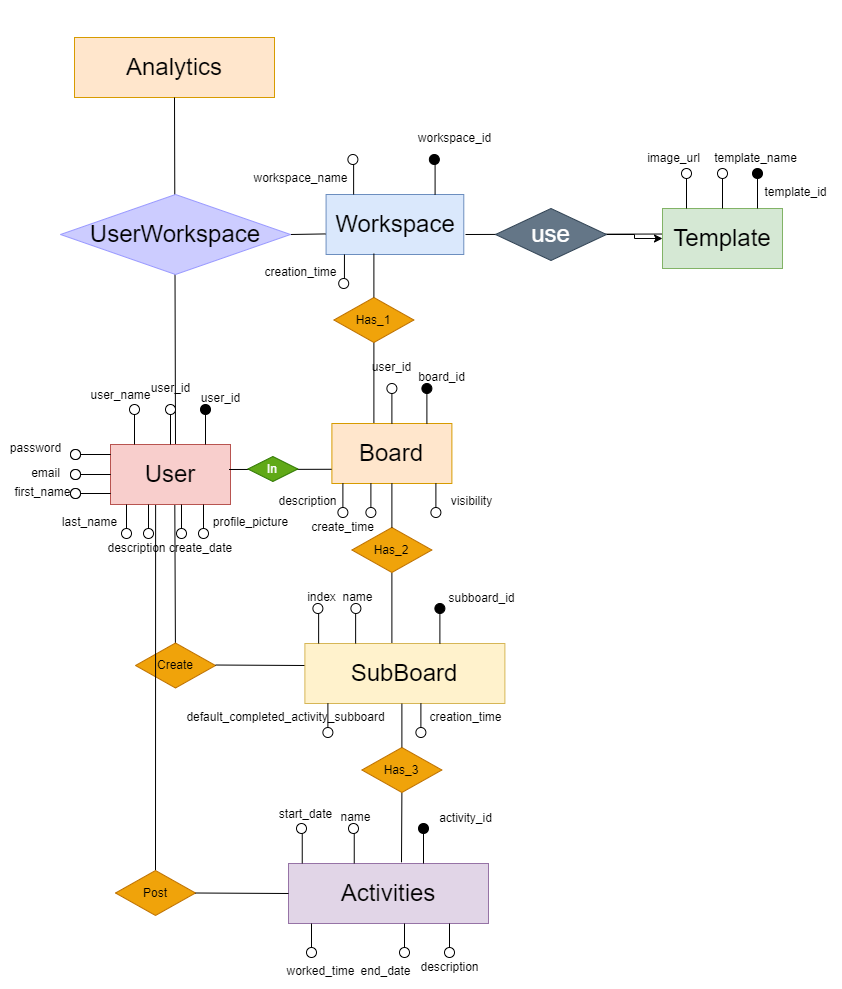
\includegraphics[width=\columnwidth]{images/ER-schma.png}

\noindent The entity-relationship contains 8 main entities:
\begin{itemize}
    \item User: each user has, as primary key, their email, which is of type char with variable length (up to 64 characters). For each user we also record their first name, last name (of type char), role (of type roles) and password. Note that the password is hashed through sha512 before storing it.
    \item Workspace: a workspace is a virtual space where teams can collaborate on projects and tasks. It is essentially a container for multiple boards, which are individual task lists that can be customized to fit the needs of specific projects or workflows. Each model is uniquely identified by a workspace-id and has a textual description and permission-name.
    \item User Workspace: the user work space is the place for controlling the users,identified by its user-id, workspace-id, permission-id.
    \item Board: a board is the main organizational unit used to manage tasks and projects and identified by board-id and has create-time, description, visibility, name.
    \item Analytics: each model of Analytics, analyze the performances of each user in working and provide report. It is identified by user-id and activity-id.
    \item Subboard: each model is a board which is sub-part of board and identified by subboard-id and has board-id and name 
    \item Activities:activities refer to the actions or events that have occurred on a board or card.it's identified by activity-id and it has subboard-id and name and description
    \item Template:a template refers to a pre-designed board setup that can be used as a starting point for creating new boards. this table has two external keys, it identified as template-id and has imag-url and image-name
\end{itemize}
